% Pohon Faktor dan Faktorisasi Prima dengan TikZ
% Kompilasi: pdflatex tikz-pohon-faktor-faktorisasi-prima.tex
\documentclass[11pt]{article}
\usepackage[margin=2cm]{geometry}
\usepackage{tikz}
\usepackage{xcolor}
\definecolor{bg}{HTML}{171D2B}
\definecolor{aksen}{HTML}{F7B538}

\begin{document}
\pagecolor{bg}
\color{white}

\section*{Pohon Faktor 60}

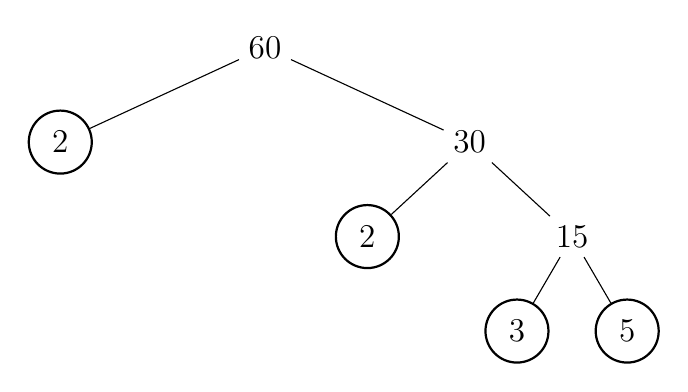
\begin{tikzpicture}[
  level distance=12mm,
  level 1/.style={sibling distance=52mm},
  level 2/.style={sibling distance=26mm},
  level 3/.style={sibling distance=14mm},
  every node/.style={font=\large},
  prime/.style={circle, draw=black, thick, minimum size=8mm},
]
\node {60}
  child { node[prime] {2} }
  child { node {30}
    child { node[prime] {2} }
    child { node {15}
      child { node[prime] {3} }
      child { node[prime] {5} }
    }
  };
\end{tikzpicture}

\section*{Faktorisasi 72 lewat Dua Jalur}

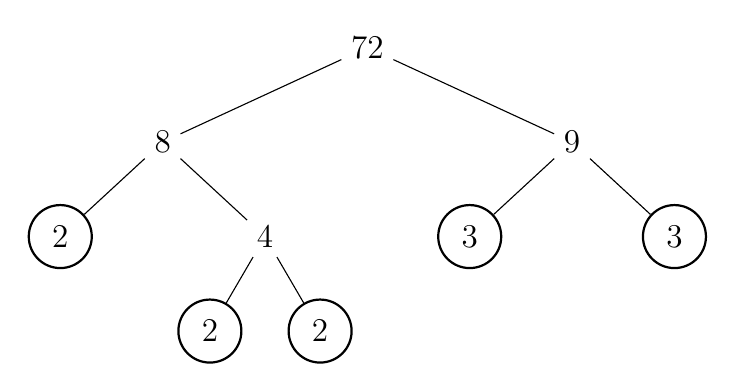
\begin{tikzpicture}[
  level distance=12mm,
  level 1/.style={sibling distance=52mm},
  level 2/.style={sibling distance=26mm},
  level 3/.style={sibling distance=14mm},
  every node/.style={font=\large},
  prime/.style={circle, draw=black, thick, minimum size=8mm},
]
\node {72}
  child { node {8}
    child { node[prime] {2} }
    child { node {4}
      child { node[prime] {2} }
      child { node[prime] {2} }
    }
  }
  child { node {9}
    child { node[prime] {3} }
    child { node[prime] {3} }
  };
\end{tikzpicture}

\qquad
\begin{tikzpicture}[
  level distance=12mm,
  level 1/.style={sibling distance=52mm},
  level 2/.style={sibling distance=26mm},
  level 3/.style={sibling distance=14mm},
  every node/.style={font=\large},
  prime/.style={circle, draw=black, thick, minimum size=8mm},
]
\node {72}
  child { node[prime] {2} }
  child { node {36}
    child { node[prime] {2} }
    child { node {18}
      child { node[prime] {2} }
      child { node {9}
        child { node[prime] {3} }
        child { node[prime] {3} }
      }
    }
  };
\end{tikzpicture}

Kedua jalur memberi hasil akhir yang sama: $2^3 \times 3^2$.

\end{document}
